\documentclass{esannV2}
\usepackage{graphicx}
\usepackage[latin1]{inputenc}
\usepackage{amssymb,amsmath,array}
\usepackage{subfigure}
\usepackage{hyperref}

%***********************************************************************
% !!!! IMPORTANT NOTICE ON TEXT MARGINS !!!!!
%***********************************************************************
%
% Please avoid using DVI2PDF or PS2PDF converters: some undesired
% shifting/scaling may occur when using these programs
% It is strongly recommended to use the DVIPS converters, and to submit
% PS file. You may submit a PDF file if and only if you use ADOBE ACROBAT
% to convert your PS file to PDF.
%
% Check that you have set the paper size to A4 (and NOT to letter) in your
% dvi2ps converter, in Adobe Acrobat if you use it, and in any printer driver
% that you could use.  You also have to disable the 'scale to fit paper' option
% of your printer driver.
%
% In any case, please check carefully that the final size of the top and
% bottom margins is 5.2 cm and of the left and right margins is 4.4 cm.
% It is your responsibility to verify this important requirement.  If these margin requirements and not fulfilled at the end of your file generation process, please use the following commands to correct them.  Otherwise, please do not modify these commands.
%
\voffset 0 cm \hoffset 0 cm \addtolength{\textwidth}{0cm}
\addtolength{\textheight}{0cm}\addtolength{\leftmargin}{0cm}

%***********************************************************************
% !!!! USE OF THE esannV2 LaTeX STYLE FILE !!!!!
%***********************************************************************
%
% Some commands are inserted in the following .tex example file.  Therefore to
% set up your ESANN submission, please use this file and modify it to insert
% your text, rather than staring from a blank .tex file.  In this way, you will
% have the commands inserted in the right place.

\begin{document}
%style file for ESANN manuscripts
\title{Deep Learning Vector Quantization}

%***********************************************************************
% AUTHORS INFORMATION AREA
%***********************************************************************
\author{Harm de Vries, Roland Memisevic and Aaron Courville
%
% Optional short acknowledgment: remove next line if non-needed
%\thanks{This is an optional funding source acknowledgement.}
%
% DO NOT MODIFY THE FOLLOWING '\vspace' ARGUMENT
\vspace{.3cm}\\
%
% Addresses and institutions (remove "1- " in case of a single institution)
Universit\'{e} de Montr\'{e}al \\
%\textit{mail@harmdevries.com}
%
% Remove the next three lines in case of a single institution
}
%***********************************************************************
% END OF AUTHORS INFORMATION AREA
%***********************************************************************

\maketitle

\begin{abstract}
We introduce an extension of Generalized Learning Vector Quantization (GLVQ), a popular prototype based classifier, that incorporates non-linear metric learning by a deep neural network. We show that our proposed extension, called Deep Learning Vector Quantization (DLVQ), outperforms the linear metric learning variant GMLVQ. Compared to the traditionally used log-softmax objective, DLVQ slighlty improves classification performance while being more robust against fooling and adversarial examples. 
\end{abstract}

\section{Introduction}
Although Deep Neural Networks (DNN's) \cite{DBLP:journals/corr/abs-1206-5538} have reached near human-level performance on challenging object recognition tasks \cite{krizhevsky2012imagenet,DBLP:journals/corr/IoffeS15}, recent studies  highlight that there remain quite some differences with the human visual system. The first intriguing observation made is that DNN's are vulnerable to \emph{adversarial examples} \cite{DBLP:journals/corr/SzegedyZSBEGF13} -- worst-case, imperceptible changes to the input that causes the DNN to label it completely different. Follow-up research \cite{DBLP:journals/corr/NguyenYC14} showed that DNN's are also easily \emph{fooled} -- we can produce images for which a DNN assigns high confidence as belonging to one of the classes while not coming from the data distribution. 

Our work departs from the observation that such fooling examples might be caused by the extrapolating nature of the log-softmax:
\begin{equation}
L_{SM} = \sum_n \log p(\hat{y}^{n}| \mathbf{x}^{(n)}) = \log \frac{\exp(w_{y^{(n)}}^\top \mathbf{x} + b_{y^{(n)}})}{\sum_i \exp(w_i^\top \mathbf{x} + b_i)},
\end{equation}
the commonly used loss function for classication problems with neural networks. We illustrate this point with an artificially generated three-class problem shown in Fig. \ref{figure:diff_glvq_softmax}. 
We can see that the softmax becomes more confident when a point is farther from the decision boundary, even though there is no data to support this decision. In contrast, a prototype based classifier like Generalized Learning Vector Quantization (GLVQ) \cite{sato1996generalized} produces only high confidence values near the data points (near the prototypes). In this paper we propose to combine deep neural networks with GLVQ. 


\section{Generalized Learning Vector Quantization}
We assume we are given training data $(\mathbf{x}^{(n)}, y^{(n)}) \in R^D \times \{0, ..., K-1\}$, $n=1, ..., N$, where $D$ is the dimensionality of the input, and $K$ the number of classes. A LVQ classifier consist of a set of prototypes ${\mathbf{w}_j} \in R^D, j=1, ..., M$ with an associated class label $c(w_j) \in \{1, ..., K\}$. In this work we consider one prototype per class, although it is straightforward to extend to multiple prototypes. Classification follows a nearest prototype scheme i.e. a new data point $\tilde{x}$ is assigned to the class of the nearest prototype $c(\mbox{arg min}_{\mathbf{w}_j} d(\tilde{x}, \mathbf{w}_j))$ according to some distance measure $d(\tilde{x}, w_j)$. 
\begin{figure}[t]
\centering{
\subfigure[Softmax]{
 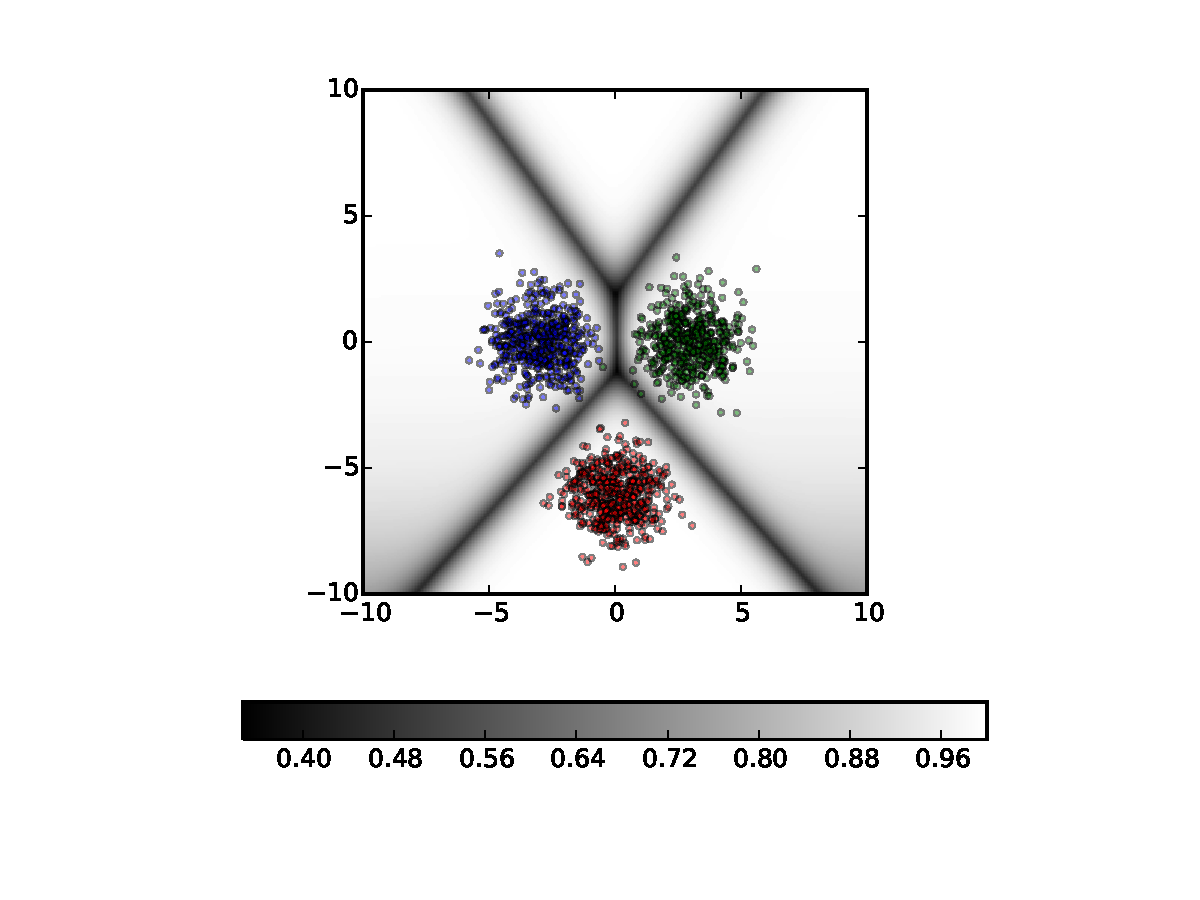
\includegraphics[width=0.48\textwidth, trim={3cm 0 1cm 0}]{../mnist/figures/softmax.pdf}}
\subfigure[GLVQ]{
 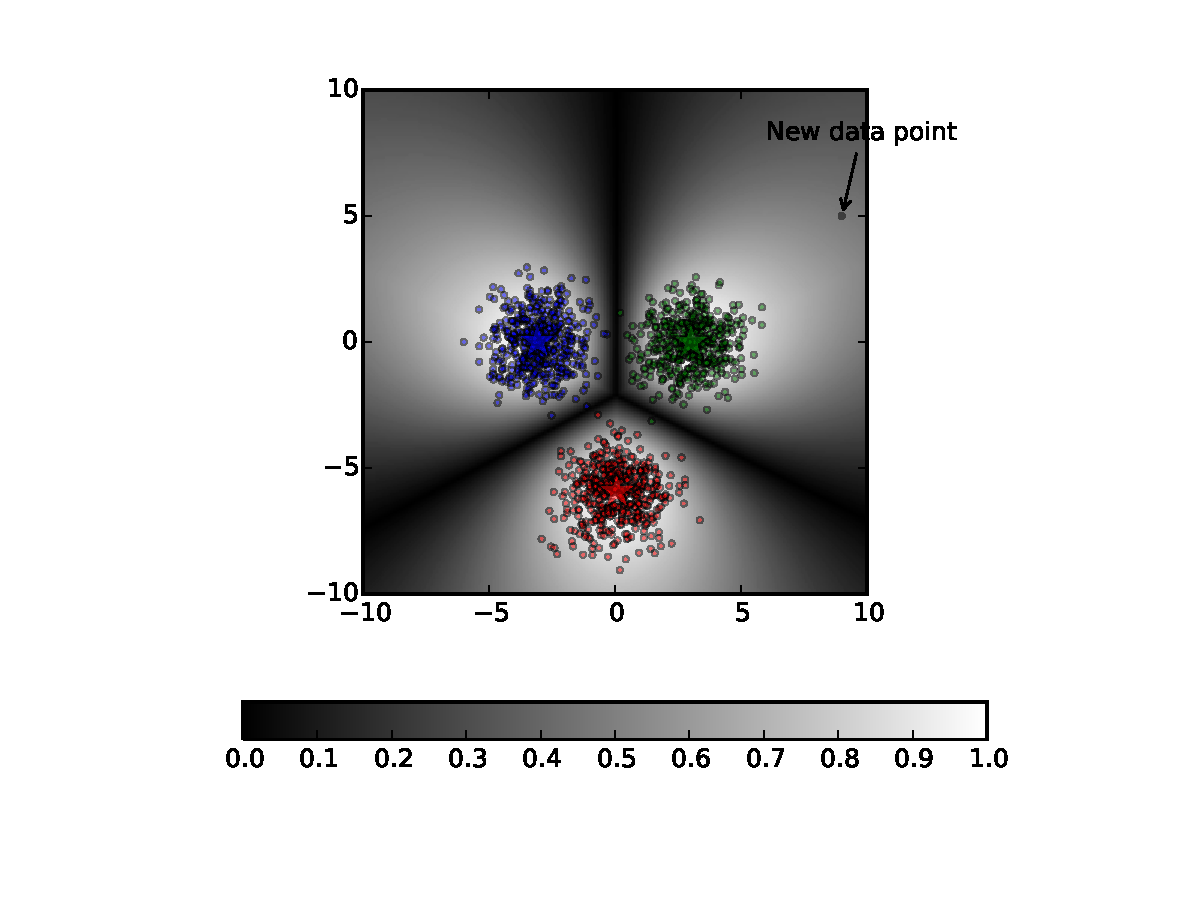
\includegraphics[width=0.48\textwidth, trim={3cm 0 1cm 0}]{../mnist/figures/lvq.pdf}}}
\caption{An artifically generated three class problem for which we have trained (a) a softmax classifier and (b) a GLVQ classifier. The background color (white for high) indicates the confidence values for a decision, that is $\mbox{arg max}_i\ p(y_j|x)$ for the softmax and $-l^{(n)}$ for the GLVQ classifier\protect\footnotemark. The softmax classifier will assign a high confidence value to a new data point in the right upper corner (far from the data), while GLVQ will not. }
\label{figure:diff_glvq_softmax}
\end{figure}
\footnotetext{We multiplied $l^{(n)}$ with $-1$ such that higher values indicates higher confidence.}

Training aims to find the locations of the prototypes such that the data points are assigned to their corresponding class labels. Generalized Learning Vector Quantization (GLVQ) \cite{sato1996generalized} aims to achieve this objective by minimizing the following training criterion:
\begin{equation}
 L_{GLVQ}(\theta) = \sum_n \phi(l^{(n)}) \mbox{~~with~~} l^{(n)} = \frac{d^{(n)}_+ - d^{(n)}_-}{d^{(n)}_+ + d^{(n)}_-}
\end{equation}
where $d^{(n)}_+ = \mbox{min}_{c(w_j) = y} d(x^{(n)}, \mathbf{w}_j)$ and $d^{(n)}_- = \mbox{min}_{c(\mathbf{w}_j)\neq y} d(x_i, \mathbf{w}_j)$ denote the distance to the closest correct and closest wrong prototype, respectively. The numerator of $l^{(n)}$ denotes the margin between the correct and wrong class, while the denominator scales the term within the interval $[-1, 1]$. The scaling function $\phi$ provides a handle to balance error minimization and margin maximization. Using the step function corresponds to the non-differentiable zero-one loss, and using the identity function corresponds to an average margin maximization. A trade-off between the two terms can be realised by a scaling function $\phi(x) = \exp(\gamma x)$, where $\gamma > 0$ controls the steepness of the exponential. 

Note that the numerator in $l^{(n)}$ is the reason why GLVQ only produces high confidence values when you are close to the data. If move away from the data we add a constant $a > 0$ to the distances $d^+$ and $d^-$, this contribution will cancel in the numerator while it will add $2a$ to the denominator. For correctly classified data points (i.e. negative terms) this will increase the cost function value.

\section{Supervised neural gas}
The main drawback of the GLVQ cost function is that it only displays correct training dynamics for correctly classified training examples\cite{sato1996generalized}.  To see this, note that for incorrectly classified examples the gradient with respect to the incorrect distance $\partial l^{(n)} / \partial d^{(n)}_- = 4d^{(n)}_+/(d^{(n)}_+ - d^{(n)})^2$ is bigger than the gradient with respect to the correct class $\partial l^{(n)} / \partial d^{(n)}_+ = -4d^{(n)}_-/(d^{(n)}_+ - d^{(n)})^2$. The repelling force on the prototypes then dominates the attractive force which leads to prototypes that diverge from the data distribution. We empirically found this to be a problem, when we initially tried to optimize a neural net with the GLVQ cost function. 

One way to alleviate this problem is not to compare against the \emph{closest} incorrect prototype, but against the \emph{average} distance to all incorrect prototypes. This smears out the repelling force over several prototypes, and makes it more likely that training dynamics are stable. This is the rationale behind Supervised Neural Gas (SNG) \cite{SNG} which minimizes the following cost function\footnote{We note two reasonable alternatives: 1) the neighborhood function can be pushed into $l^{(n)}$ i.e. we define $d^{(n)}_- = \sum_{j \neq y^{(n)}} h_\tau(x^{(n)}, j) d(x^{(n)}, \mathbf{w}_j)$ and 2) the neighborhood function can also be replaced by a softargmin $h_\tau(x^{(n)}, j) = \exp(-\tau d(x, w_j)/\sum_k \exp(-\tau d(x^{(n)}, \mathbf{w}_k))$}:
\begin{equation}
 L_{SNG} = \sum_n \sum_{j\neq y^{(n)}} h_\tau(x^{(n)}, j) \phi\left(\frac{d^{(n)}_+ - d(x^{(n)}, \mathbf{w}_j)}{d^{(n)}_+ + d(x^{(n)}, \mathbf{w}_j)}\right)
\end{equation}
The neighborhood function $h_\tau(x^{(n)}, j) = \exp(-\tau k_j)/ \sum_{k=0}^{K-1} \exp(-\tau k)$ determines a (normalized) weight for each incorrect prototype loss that depends on its rank $k_j$, the number of prototypes that are closer to the considered data point. Our training strategy is to start with small $\tau \rightarrow 0$, essentially averaging over all incorrect prototypes, and slowly increase $\tau \rightarrow \infty$ such that we recover the GLVQ cost function. 

% There are two other important observation to make about the cost function: 
% \begin{itemize}
% \item The loss is invariant to the scale of the distances. That is, if each distance is multiplied by some constant $c \neq 0$\footnote{The closest correct and closest wrong prototype don't change}, the corresponding cost function value remains the same. 
% \item The loss is sensitive to an additive term. That is, if we add some constant $a > 0$ to the distances $d^+$ and $d^-$, this contribution will cancel in the numerator while it will add $2a$ to the denominator. For correctly classified data points (i.e. negative terms) this will increase the cost function value.          
% \end{itemize} 
% In summary, the first bullet point points out that we are maximizing a \emph{scale-invariant} margin. The second point is important to provide low confidence values far away from the data as will be explained in the next section. 

\section{Deep LVQ}
It is possible to use any differentiable distance function $d$ within the SNG and GLVQ cost functions. We propose to parameterize the distance function as:
\begin{equation}
 d(\mathbf{x}, \mathbf{w}_j) = \|f(\mathbf{x}; \theta) - \mathbf{w}_j\|^2_2
\end{equation}
where $f$ is a deep neural network with parameters $\mathbf{\theta}$ that non-linearly projects the data points into an embedding space. During training we jointly optimize the neural net parameters $\theta$ and the prototypes $W$. 

Note that a linear projection $f(x) = Ax$ boils down to Generalized Matrix Learning Vector Quantization (GMLVQ) \cite{schneider2009adaptive,bunte2012limited}. A notable difference with that work is that we directly parameterize the prototypes in embedding space. This saves computational time because we avoid a forward pass through the neural network $f$ for the prototypes. Although the prototypes are no longer directly\footnote{The prototypes can be projected back to input space after training} interpretable as class conditional exemplars in input space, recent work\cite{de2013stationarity} has shown that such an interpretation is problematic. Due to the tendency of the GLVQ cost function to learn an injective (many-to-one) mapping $f$, the prototypes can only be considered class-conditional representatives in the embedding space. 


\section{Experiments}
\begin{table}
\caption{Classification results on MNIST for a feedforward net with GLVQ and softmax cost function. We compare without regularization, with batch normalization (BN), and input noise. We also report results for GMLVQ with $1$ and $10$ prototypes per class. Results are average test error over 3 runs, standard deviation is reported between parentheses. }
\label{table:results}
 \begin{tabular}{l||llll}
  & Softmax & DLVQ & GMLVQ(1) & GMLVQ (10)\\
 \hline
 No regularization & 1.73 (0.02) & 1.28 (0.07) & 8.21 (0.01) & 5.01 (0.03)\\
 BN & 1.31 (0.03) & 1.22 (0.02)& &\\
 BN + input noise & 1.05 (0.02) & 0.98 (0.03)&&
 \end{tabular}
\end{table}

\subsection{MNIST}
The MNIST dataset consist of 70,000 handwritten digits ranging from $0$ to $9$. We make the usual split of $50,000$, $10,000$ and $10,000$ for the training, validation and test set, respectively. We divide the images by $255$ to scale the pixels within $[0, 1]$.  We use a fully connected neural network with $1200-1200-200$ hidden units, followed by either a log softmax or GLVQ. All units have rectified linear activations. We initialize the prototypes for DLVQ as the class conditional means in the embedding space. We start training with a large neighborhood, i.e. $\tau=0.1$, and linearly increase to $\tau=30.0$. 
We trained our networks for $100$ epochs with ADAM \cite{DBLP:journals/corr/KingmaB14}, and present the test errors by early stopping on the validation error.  
Our code is implemented in Theano \cite{Bastien-Theano-2012}, and is available at \url{https://github.com/harmdevries89/lvq}. 


We compare training without any form of regularization, with batch normalization (BN) \cite{DBLP:journals/corr/IoffeS15}, and additive gaussian noise of standard deviation $0.5$ on the inputs. The results are shown in Table \ref{table:results}. Without any form of regularization, DLVQ significantly outperforms the softmax. This gap reduces when we use batch normalization, which has a better regularization effect for the softmax. When we also include input noise, DLVQ still outperforms the softmax and reaches a notable $0.98\%$ test error. 

We also compare DLVQ to GMLVQ with $1$ and $10$ prototypes per class. Unsurpisingly, the linear transformation does not have enough capacity resulting in poor performance of $8.2\%$. Even increasing the number of prototypes from $1$ to $10$ only slightly improved the performance to $5.0\%$, clearly worse than DLVQ. 

\subsubsection{Fooling and adversarial examples}
We verify if DLVQ is more robust against fooling examples than the softmax. As a first test we measure how confident the classifier is when we feed it $10,000$ data points sampled from large uniform noise $\mathcal{U}(-10.0, 10.0)^{784}$. A histogram of the resulting confidence values is shown in Fig. \ref{fig:confidence} For the softmax, the confidence values are indistinguishable from the produced confidences on the . As expected,  inputting large input values automatically \emph{fools} a neural network. On the other hand, DLVQ is robust against such outliers by construction.

This automatically raises the questions if DLVQ is not vulnerable to other fooling examples. 


\begin{figure}[t]
\centering{
\subfigure[Softmax]{
 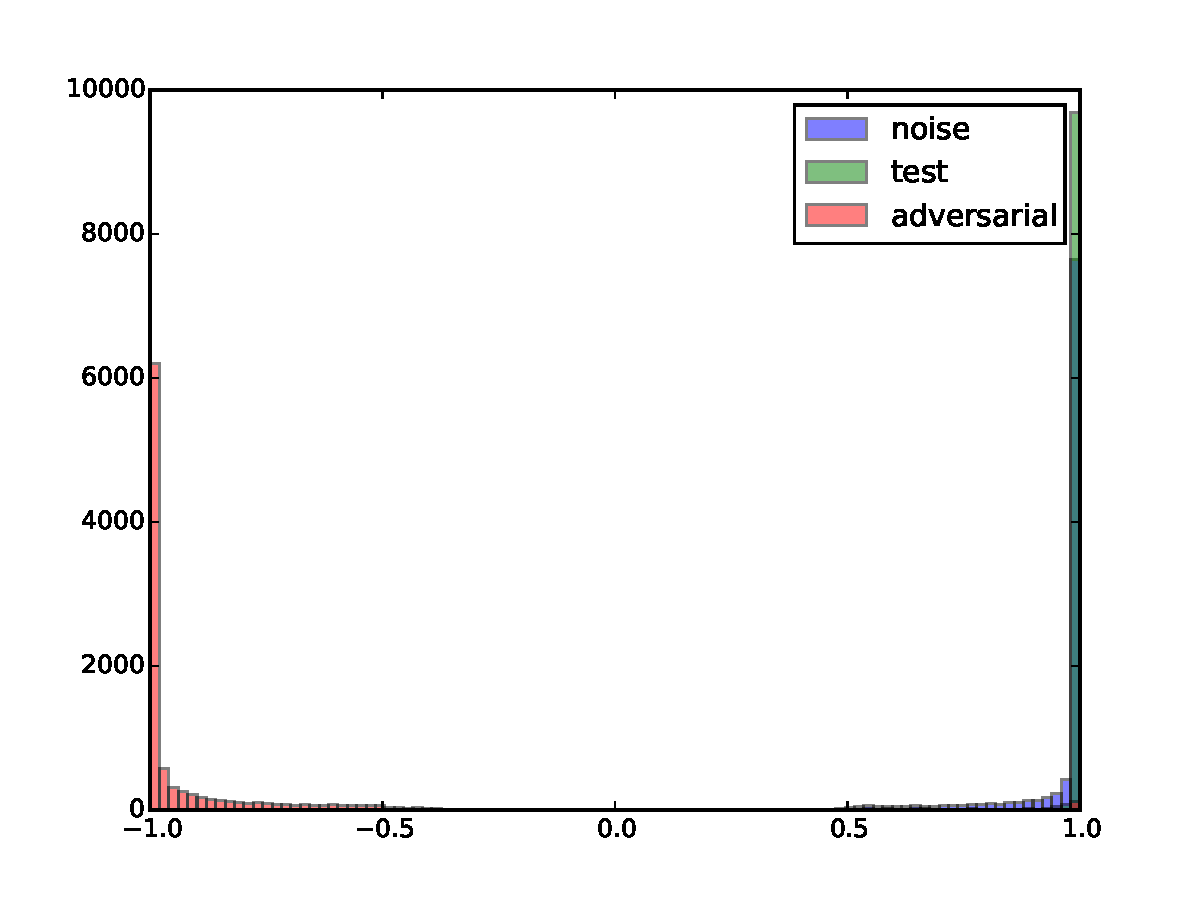
\includegraphics[width=0.48\textwidth]{../mnist/figures/softmax_conf.pdf}}
\subfigure[DLVQ]{
 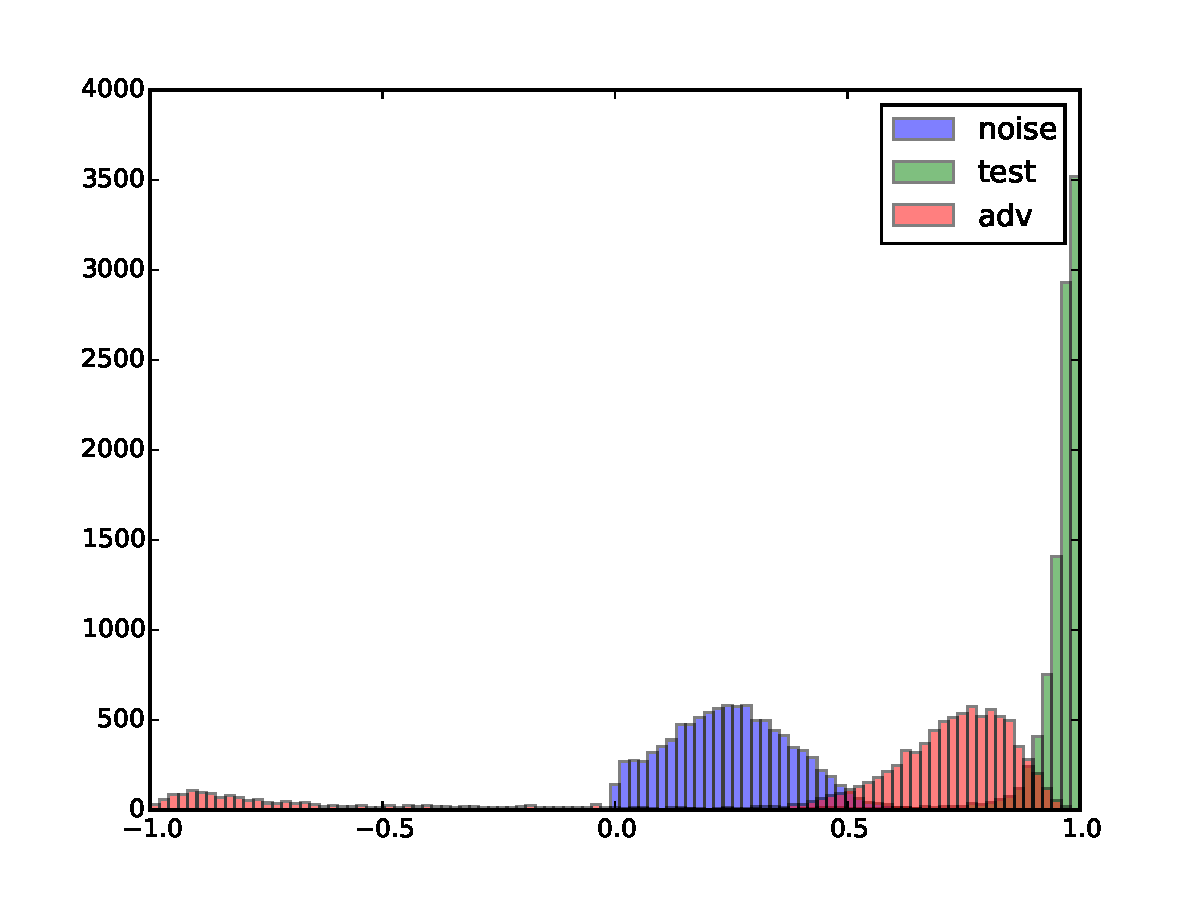
\includegraphics[width=0.48\textwidth]{../mnist/figures/lvq_conf.pdf}}}
\caption{Histogram of the confidence values for the neural network trained with a) softmax and b) GLVQ on MNIST. The green bars indicate the confidence values for the test set, the blue bars indicate the confidence values for noise drawn from $\mathcal{U}(-10, 10)^{784}$ and the red bars denote the confidence for adversarial examples on the test set.}
\label{fig:confidence}
\end{figure}

%9551
%1195

\begin{figure}[t]
\centering{
 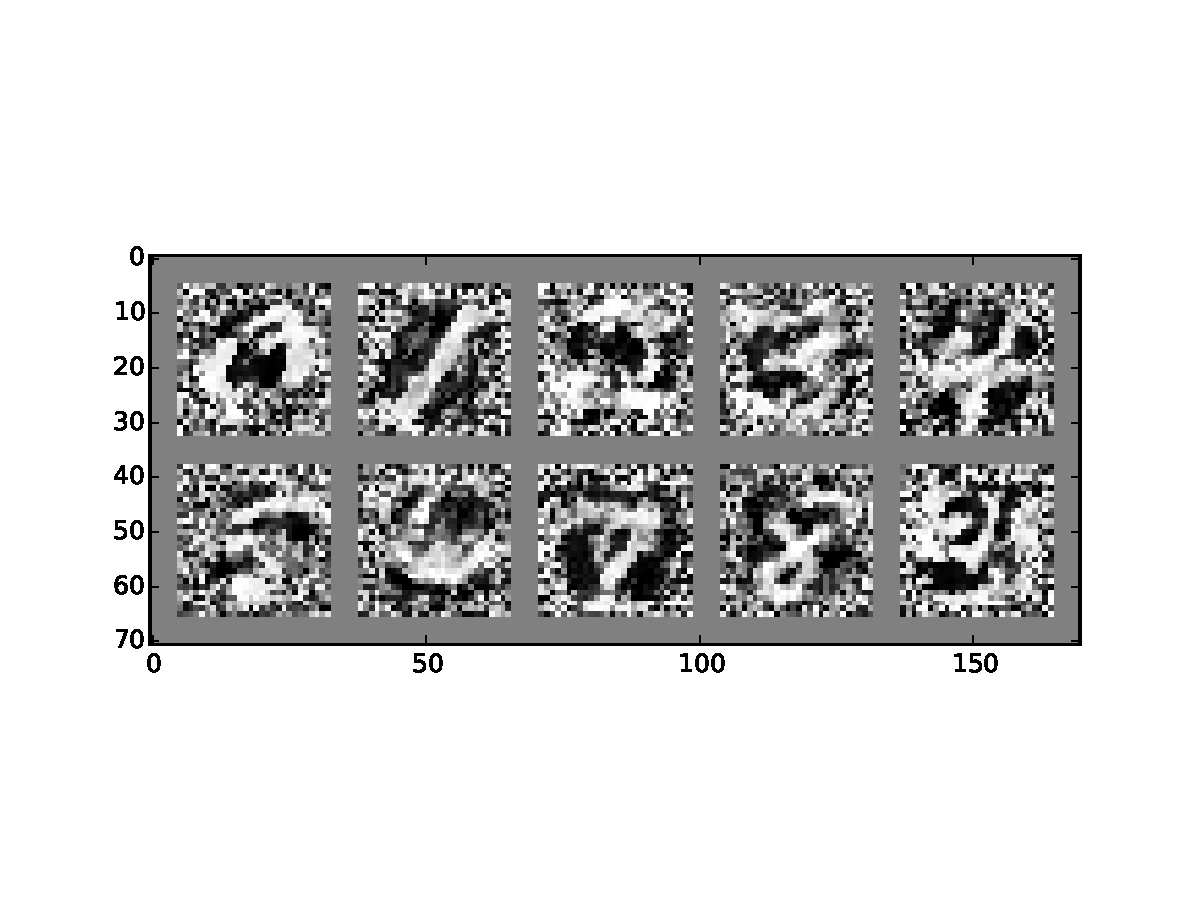
\includegraphics[width=0.48\textwidth]{../mnist/figures/fooling.pdf}}
}
\caption{}
\label{fig:fooling}
\end{figure}

\section{Conclusion}

% ****************************************************************************
% BIBLIOGRAPHY AREA
% ****************************************************************************

\begin{footnotesize}

% IF YOU USE BIBTEX,
% - DELETE THE TEXT BETWEEN THE TWO ABOVE DASHED LINES
% - UNCOMMENT THE NEXT TWO LINES AND REPLACE 'Name_Of_Your_BibFile'

\bibliographystyle{unsrt}
\bibliography{refs}

\end{footnotesize}

% ****************************************************************************
% END OF BIBLIOGRAPHY AREA
% ****************************************************************************
%\appendix
%\section{Softmax follows from gaussian class-conditionals}
%Let's assume that the class-conditional distribution $p(x|y_j) = \frac{1}{Z} \exp(-\frac{1}{2\sigma^2}(\mathbf{x} - \mathbf{w}_j)^{\top}(\mathbf{x} - \mathbf{w}_j))$ is an isotropic Gaussian distribution with normalization constant $Z = ..$. 

\end{document}
